\documentclass[12pt]{article}
\usepackage{setspace, graphicx, fullpage, amssymb, amsmath, epsfig, natbib, array, multirow, hyperref}
\usepackage{amsfonts, bm} 
\usepackage{dcolumn}
\usepackage{subfigure, float} 
\usepackage[margin=1in]{geometry} 
\usepackage{verbatim}
\usepackage{url}
\usepackage{enumerate}
\usepackage{morefloats}
\newcolumntype{d}[1]{D{.}{.}{#1}} 



\begin{document}
	
\begin{center}
	\Large 22 March 2017
\end{center}

\section{Overview}

At our previous meeting we decided to do the following:

\begin{itemize}
	\item Begin work on framing/writing an article about the role of reelection in party calls and noncalls
	
	\item Work with subgroups in the nonparametric analyses, especially separating cases of states with different party Senators by which is up for reelection; work to come up with explanations of why we see what we see
	
	\item Redo intra-party coefficient plots to focus on Congresses in which subgroups 
	
	\item Present DV/IV plots for Republicans and Democrats, the Majority and Minority caucuses, and combinations thereof
\end{itemize}

\noindent
These are included below. Note that I multiplied the vote share variable in the Senate by 100 so that it would be more similar to the vote percent variable in the House.

\section{First Stab at Reelection Paper}

\subsection{Introduction}

In this paper, we provide a replication of Minozzi \& Volden (2013). The paper we are replicating separates roll call votes into ``party calls'' and ``non party calls'' based on the ability of vote choice to be predicted by ideology. Roll call votes from Congresses 93-109 in the House of Representatives were used. This was then used to test the hypothesis that more ideologically extreme members of Congress were more responsive than their moderate counterparts.

This paper works to replicate these findings and extend them into more recent Congresses in the House as well as into the Senate for these Congresses. Extending into the Senate allows us not only to see if members respond to the party in the Senate as they do in the House, but also to test the role of proximity to reelection in members' behavior. As with much work considering the behavior of members of Congress, we begin with the assumption that chief among a member's goals is reelection (Mayhew, 1974). While this would seem to indicate that members would act according to the preferences of their district above those of their party, we know from Lee (2009) that the name brands of parties confer advantages on members and that members are thus willing to take actions and positions that are either beneficial to their own party relative to the opposition. However, we also know from Carson, Koger, Lebo \& Young (2010) that following the party line too closely can be electorally costly to an individual member. It is therefore worth considering whether proximity to election changes the costs and benefits of aiding the party as perceived by members. Levitt (1996) finds members' behavior (as proxied by ADA score) is less a factor of the party (as proxied by party leaders) and more of those of their home state (as proxied by the average ADA score of House members from their state). While these results are highly persuasive and indicative of general aspects of the decision-making process of Senators approaching reelection, what is missing is trends in member behavior relating to party influence. 

Members would most credibly signal to constituents that they are not mere obedient partisans by voting opposite the party on key votes. While perhaps the most effective route available to them, this would also cause the most damage to the goals of the party. It remains possible that instead members behave differently on votes less influenced by the party in order to differentiate themselves in these years in order to still aid the party while still allowing themselves to stake out a claim of being more than a mere partisan. Alternately, it could be the case that only certain types of members of Congress (those electorally at risk, for instance) choose to buck the party in this way, or that such action does not occur in any meaningful way. 

Still, we must first establish whether Senators behave similarly to Representatives on party call votes. To this end, we show the results of our replication and provide a discussion of the results. This is followed by analysis which discusses the electoral connection in the Senate. In order to analyze this, we conduct a number of tests aimed at testing the influence of reelection within members. The first of these uses same-state Senators as a natural matched pair, following Levitt (1996), while the second estimates a fixed effects model to consider within member variation resulting from reelection. We find that reelection causes members to vote against their party more on party call votes but not other votes.

\subsection{Replication: Party Calls in the House and Senate}

In this section we show that the results from Minozzi \& Volden (2013) hold when analysis is included for later Congresses in the House as well as those Congresses Senate. We draw on Congressional roll call data for Congresses 93-112 for both chambers in order to view the behavior of members. As in Minozzi \& Volden (2013), we iteratively sort votes based on the the predictive power of party in vote decision taken alongside party free ideology. We dub those votes which are significantly predicted by party as party calls and those which are not as noncalls. The set of noncalls from one iteration is used as the votes for calculating party free ideology in the next. As in the paper we are replicating, we drop votes which have their categorization switch in the last 5 iterations. We use this to form our main dependent and independent variables, responsiveness to party calls, baseline rate of voting with a majority of the party (on noncalls), and ideological extremism (party free ideology with sign inversed for Democrats).

We have made some changes to the sorting algorithm used to sort votes. One of the key changes was the use of the \verb|emIRT()| R function as described in Imai, Lo \& Olmsted (2016) in order to obtain members' party free ideology. This function was developed by those authors in order to produce estimates analagous to those of the \verb|ideal()| function developed by Clinton, Jackman \& Rivers (2004) and used in the prior party call sorting algorithm. A key advantage of this new function for estimation of member ideology is that it produces results with greatly reduced computation. These and other changes, as detailed in an appendix, produce highly similar results to those found in Minozzi \& Volden (2013) when applied to both chambers. We find for each chamber that party call votes are more often close votes and the opposite holds for noncalls. Votes are considered lopsided when at least 65\% of members vote the same way on it and close otherwise. 

% latex table generated in R 3.3.2 by xtable 1.8-2 package
% Mon Mar 20 13:02:44 2017
\begin{table}[H]
	\centering
	\caption{House Vote Coding for Close and Lopsided Votes} 
	\begin{tabular}{lrr}
		\hline
		& Party Call & Noncall \\ 
		\hline
		Lopsided & 4245 & 6123 \\ 
		Close & 9308 & 1090 \\ 
		\hline
	\end{tabular}
\end{table}

% latex table generated in R 3.3.2 by xtable 1.8-2 package
% Mon Mar 20 13:04:18 2017
\begin{table}[H]
	\centering
	\caption{Senate Vote Coding for Close and Lopsided Votes} 
	\begin{tabular}{lrr}
		\hline
		& Party Call & Noncall \\ 
		\hline
		Lopsided & 2063 & 4876 \\ 
		Close & 5233 & 1851 \\ 
		\hline
	\end{tabular}
\end{table}

Further, pooled regressions with members divided by party and majority status broadly show similar relationships both between chambers in the current analysis as well as with those presented in Minozzi \& Volden (2013). Information regarding the construction and summary statistics of variables used in this paper will be included in an appendix. Though they differ in strength between parties, ideological extremism and rate of voting with majority of non party call votes both carry substantive predictive power in determining responsiveness by to party calls. Unsurprisingly, in both chambers we also find that southern Democrats are less responsive to the party than are other Democrats.

As previously stated, conducting analyses in the Senate allows us to consider the roll of election proximity on member response to party calls. The indicator variable shows a decrease in responsiveness across the groups found in our pooled regression analysis. We note that this relationship is reduced both in terms of substantive effect and statistical significance for Democrats up for reelection in the pooled analysis. The sign remains the same for Democrats, however. One possibility for this is that political parties and party unity are less popular among Republicans than Democrats, thus leading to different effect sizes. While the pooled regression shows that the trend is for members to be less responsive to the call of the party in Congresses which they are up for reelection, it is possible that there are unobserved factors that vary among members or across time which are responsible for the relationship we see with the indicator for up for reelection. We seek to test this possibility in the coming section.

\begin{table}[H]
	\begin{center}
		\caption{Responsiveness to Party Calls in the House}
		\begin{tabular}{l c c c c }
			\hline
			& Democrats & Republicans & Majority & Minority \\
			\hline
			Ideological Extremism & $8.34^{***}$  & $5.84^{***}$  & $6.65^{***}$  & $8.73^{***}$  \\
			& $(0.17)$      & $(0.21)$      & $(0.16)$      & $(0.20)$      \\
			Baseline Rate of Voting with Party              & $0.64^{***}$  & $0.41^{***}$  & $0.52^{***}$  & $0.64^{***}$  \\
			& $(0.02)$      & $(0.02)$      & $(0.01)$      & $(0.02)$      \\
			Vote Percent                & $-0.04^{***}$ & $-0.00$       & $-0.09^{***}$ & $-0.07^{***}$ \\
			& $(0.01)$      & $(0.01)$      & $(0.01)$      & $(0.01)$      \\
			President Vote Percent          & $0.09^{***}$  & $-0.09^{***}$ & $0.20^{***}$  & $0.16^{***}$  \\
			& $(0.01)$      & $(0.02)$      & $(0.01)$      & $(0.02)$      \\
			South                  & $-2.43^{***}$ & $3.63^{***}$  & $-1.64^{***}$ & $-0.38$       \\
			& $(0.28)$      & $(0.34)$      & $(0.25)$      & $(0.31)$      \\
			Female                 & $0.53$        & $-0.08$       & $-0.14$       & $2.12^{***}$  \\
			& $(0.35)$      & $(0.57)$      & $(0.40)$      & $(0.44)$      \\
			African American                   & $-0.52$       & $5.01$        & $-3.04^{***}$ & $3.25^{***}$  \\
			& $(0.44)$      & $(2.97)$      & $(0.53)$      & $(0.61)$      \\
			Latino                 & $1.73^{***}$  & $2.41^{*}$    & $2.82^{***}$  & $3.02^{***}$  \\
			& $(0.51)$      & $(1.15)$      & $(0.63)$      & $(0.70)$      \\
			Seniority              & $0.05$        & $-0.33^{***}$ & $0.01$        & $0.01$        \\
			& $(0.03)$      & $(0.05)$      & $(0.03)$      & $(0.04)$      \\
			Freshman               & $-0.07$       & $1.00^{*}$    & $0.24$        & $-0.41$       \\
			& $(0.36)$      & $(0.46)$      & $(0.35)$      & $(0.45)$      \\
			Best Committee         & $-0.04^{*}$   & $-0.24^{***}$ & $-0.18^{***}$ & $-0.16^{***}$ \\
			& $(0.02)$      & $(0.03)$      & $(0.02)$      & $(0.02)$      \\
			Party Leader                 & $1.96^{**}$   & $2.80^{***}$  & $2.61^{***}$  & $1.78^{**}$   \\
			& $(0.60)$      & $(0.76)$      & $(0.65)$      & $(0.65)$      \\
			Power Committee                & $1.82^{***}$  & $2.95^{***}$  & $3.02^{***}$  & $1.06^{**}$   \\
			& $(0.28)$      & $(0.37)$      & $(0.27)$      & $(0.36)$      \\
			Committee Chair                  & $2.49^{***}$  & $9.85^{***}$  & $1.86^{***}$  &               \\
			& $(0.50)$      & $(0.80)$      & $(0.44)$      &               \\
			(Intercept)            & $24.00^{***}$ & $53.04^{***}$ & $36.45^{***}$ & $17.69^{***}$ \\
			& $(1.58)$      & $(2.21)$      & $(1.49)$      & $(2.05)$      \\
			\hline
			R$^2$                  & 0.63          & 0.30          & 0.57          & 0.48          \\
			Adj. R$^2$             & 0.63          & 0.30          & 0.57          & 0.48          \\
			Num. obs.              & 4746          & 3798          & 4898          & 3646          \\
			RMSE                   & 7.36          & 8.87          & 7.54          & 8.02          \\
			\hline
			\multicolumn{5}{l}{\scriptsize{$^{***}p<0.001$, $^{**}p<0.01$, $^*p<0.05$}}
		\end{tabular}
	\end{center}
\end{table}

\begin{table}[H]
	\begin{center}
		\caption{Responsiveness to Party Calls in the Senate}
		\begin{tabular}{l c c c c }
			\hline
			& Democrats & Republicans & Majority & Minority \\
			\hline
			Ideological Extremism & $3.136^{***}$  & $7.792^{***}$   & $4.708^{***}$  & $7.949^{***}$ \\
			& $(0.409)$      & $(0.357)$       & $(0.315)$      & $(0.400)$     \\
			Baseline Rate of Voting with Party              & $0.759^{***}$  & $0.742^{***}$   & $0.702^{***}$  & $0.702^{***}$ \\
			& $(0.030)$      & $(0.031)$       & $(0.025)$      & $(0.035)$     \\
			Up For Reelection    & $-0.630$       & $-1.436^{**}$   & $-0.951^{*}$   & $-1.204^{*}$  \\
			& $(0.426)$      & $(0.538)$       & $(0.411)$      & $(0.603)$     \\
			Vote Share            & $-0.053^{*}$  & $0.149^{***}$  & $-0.012$       & $0.076^{*}$   \\
			& $(0.022)$     & $(0.028)$      & $(0.021)$      & $(0.030)$     \\
			Presidential Vote Share       & $0.234^{***}$ & $-0.134^{***}$ & $0.182^{***}$  & $0.006$       \\
			& $(0.024)$     & $(0.031)$      & $(0.020)$      & $(0.032)$     \\
			South                  & $-1.690^{**}$  & $0.872$         & $0.054$        & $1.085$       \\
			& $(0.557)$      & $(0.578)$       & $(0.427)$      & $(0.622)$     \\
			Female                 & $1.690^{*}$    & $0.451$         & $0.532$        & $4.256^{***}$ \\
			& $(0.730)$      & $(1.132)$       & $(0.758)$      & $(1.113)$     \\
			African American                   & $-1.164$       & $-10.789^{*}$   & $1.531$        & $-5.519$      \\
			& $(2.789)$      & $(4.278)$       & $(4.184)$      & $(3.219)$     \\
			Latino                 & $1.814$        & $7.264^{**}$    & $4.781^{*}$    & $6.253$       \\
			& $(2.198)$      & $(2.779)$       & $(1.878)$      & $(3.506)$     \\
			Seniority              & $0.041$        & $-0.024$        & $0.077$        & $0.118$       \\
			& $(0.052)$      & $(0.072)$       & $(0.060)$      & $(0.070)$     \\
			Freshman               & $0.769$        & $0.358$         & $0.600$        & $0.996$       \\
			& $(0.708)$      & $(0.842)$       & $(0.631)$      & $(1.032)$     \\
			Retiree                & $1.599$        & $2.290^{*}$     & $1.816^{*}$    & $2.575^{*}$   \\
			& $(0.897)$      & $(0.997)$       & $(0.850)$      & $(1.110)$     \\
			Best Committee        & $0.237$        & $0.008$         & $0.027$        & $0.373^{*}$   \\
			& $(0.124)$      & $(0.154)$       & $(0.118)$      & $(0.174)$     \\
			Party Leader                 & $2.218^{**}$   & $0.910$         & $1.441^{*}$    & $1.940^{*}$   \\
			& $(0.712)$      & $(0.776)$       & $(0.661)$      & $(0.899)$     \\
			Power Committee       & $-0.855$       & $-0.325$        & $-0.052$       & $-1.468$      \\
			& $(0.772)$      & $(0.924)$       & $(0.719)$      & $(1.064)$     \\
			Chair                  & $0.852$        & $3.626^{***}$   & $-0.017$       &               \\
			& $(0.543)$      & $(0.700)$       & $(0.517)$      &               \\
			(Intercept)            & $9.447^{**}$   & $18.182^{***}$  & $16.365^{***}$ & $10.799^{**}$ \\
			& $(2.906)$      & $(3.489)$       & $(2.644)$      & $(4.009)$     \\
			\hline
			R$^2$                  & 0.689          & 0.641           & 0.684          & 0.615         \\
			Adj. R$^2$             & 0.684          & 0.635           & 0.679          & 0.608         \\
			Num. obs.              & 1042           & 951             & 1052           & 843           \\
			RMSE                   & 6.118          & 7.255           & 5.865          & 7.749         \\
			\hline
			\multicolumn{5}{l}{\scriptsize{$^{***}p<0.001$, $^{**}p<0.01$, $^*p<0.05$}}
		\end{tabular}
	\end{center}
\end{table}
 

\subsection{Extension: The Senate and Reelection}

In this section we estimate models which account for variation within members. The first tests compare the effects of being up for reelection on responsiveness to party calls and baseline rate of voting with the party through a non-parametric test. This test approximates a difference in differences test, relying on same-state Senator pairs with one member of the pair up for reelection and one not. We report these in separate tables which contain an estimated effect as well as the upper and lower bounds of 95\% bootstrapped confidence intervals for the reelection treatment and a randomly assigned ``placebo'' treatment. No controls are included in these models beyond comparison of same-state Senators. 

We use these tests to show that member behavior differs meaningfully in regard to party call votes and not noncall votes when they are up for reelection. The strength of this relationship is consistent with that found among groups (other than Democrats) in the pooled regressions found in the previous section.



% latex table generated in R 3.3.2 by xtable 1.8-2 package
% Mon Mar 20 12:45:07 2017
\begin{table}[H]
	\centering
	\caption{Reelection and Baseline Rate of Voting with Part, Difference in Differences} 
	\begin{tabular}{llrrr}
		\hline
		Test & Dependent Variable & Estimate & Lower Bound & Upper Bound \\ 
		\hline
		Effect & Baseline Rate of Voting with Party & -0.297 & -0.735 & 0.138 \\ 
		Placebo & Baseline Rate of Voting with Party & -0.312 & -1.057 & 1.067 \\ 
		\hline
	\end{tabular}
\end{table}

% latex table generated in R 3.3.2 by xtable 1.8-2 package
% Mon Mar 20 12:37:31 2017
\begin{table}[H]
	\centering
	\caption{Reelection and Response to Party Calls, Difference in Differences} 
	\begin{tabular}{llrrr}
		\hline
		Test & Dependent Variable & Estimate & Lower Bound & Upper Bound \\ 
		\hline
		Effect & Responsiveness to Party Calls & -1.569 & -2.094 & -0.996 \\ 
		Placebo & Responsiveness to Party Calls & -0.604 & -1.282 & 1.285 \\ 
		\hline
	\end{tabular}
\end{table}

We further conduct analysis with member level fixed effects in order to view how members differ in responsiveness to party calls in Congresses which they are up for reelection, controlling for unobserved differences between members and Congresses. Again, results from this model are consistent with those found in the pooled regression and non-parametric tests. The dependent variable Party Call Response Rate is a variable which ranges from 0 to 100 based on the percent of times a member votes in line with her party. Given that the average number of party calls in a Congress during the time we analyze is approximately 365. This means a Democratic Senator in a Congress which will break with her party on approximately 2 such votes whereas a Republican Senator will do so on roughly 5. While these numbers may seem small at the individual level, taken in aggregate this means that Senators will be less able to count on co-partisans nearing election on key close votes.

\begin{table}[H]
	\begin{center}
		\caption{Senate Fixed Effects Models, Party Call Response Rate}
		\begin{tabular}{l c c c c }
			\hline
			& Democrats & Republicans & Majority & Minority \\
			\hline
			Ideological Extremism  & $2.88^{***}$ & $4.00^{***}$  & $1.80^{**}$   & $3.93^{***}$ \\
			& $(0.69)$     & $(0.75)$      & $(0.64)$      & $(0.97)$     \\
			Baseline Rate of Voting with Party               & $0.37^{***}$ & $0.25^{***}$  & $0.37^{***}$  & $0.18^{*}$   \\
			& $(0.05)$     & $(0.05)$      & $(0.05)$      & $(0.07)$     \\
			Up For Reelection     & $-0.55^{*}$  & $-1.55^{***}$ & $-1.02^{***}$ & $-1.04^{**}$ \\
			& $(0.27)$     & $(0.34)$      & $(0.28)$      & $(0.37)$     \\
			Vote Share             & $0.03$       & $-0.05$       & $0.02$        & $-0.02$      \\
			& $(0.02)$     & $(0.03)$      & $(0.03)$      & $(0.04)$     \\
			Presidential Vote Share       & $0.27^{***}$ & $0.09$        & $0.31^{***}$  & $0.14^{*}$   \\
			& $(0.04)$     & $(0.05)$      & $(0.06)$      & $(0.06)$     \\
			Freshman                & $0.71$       & $0.98^{*}$    & $0.77$        & $0.78$       \\
			& $(0.48)$     & $(0.46)$      & $(0.46)$      & $(0.76)$     \\
			Retiree                 & $0.25$       & $0.88$        & $0.36$        & $0.75$       \\
			& $(0.83)$     & $(0.83)$      & $(0.99)$      & $(0.91)$     \\
			Best Committee         & $0.14$       & $0.11$        & $0.29$        & $0.36^{*}$   \\
			& $(0.12)$     & $(0.16)$      & $(0.15)$      & $(0.18)$     \\
			Power Committee        & $-0.48$      & $-0.22$       & $-1.26$       & $-0.45$      \\
			& $(0.70)$     & $(0.98)$      & $(0.89)$      & $(1.01)$     \\
			Leader                  & $0.87$       & $1.46^{*}$    & $1.39$        & $1.31$       \\
			& $(0.47)$     & $(0.62)$      & $(0.78)$      & $(0.80)$     \\
			Committee Chair                   & $0.38$       & $0.65$        & $-0.57$       &              \\
			& $(0.64)$     & $(0.71)$      & $(0.56)$      &              \\
			\hline
			Num. obs.               & 1042         & 951           & 1052          & 843          \\
			R$^2$ (full model)      & 0.89         & 0.91          & 0.92          & 0.94         \\
			R$^2$ (proj model)      & 0.26         & 0.19          & 0.31          & 0.17         \\
			Adj. R$^2$ (full model) & 0.87         & 0.88          & 0.89          & 0.91         \\
			Adj. R$^2$ (proj model) & 0.09         & -0.02         & 0.02          & -0.21        \\
			\hline
			\multicolumn{5}{l}{\scriptsize{$^{***}p<0.001$, $^{**}p<0.01$, $^*p<0.05$}}
		\end{tabular}
	\end{center}
\end{table}

\subsection{Conclusion}

In this paper, we show that members respond to party influence in the Senate as they do in the House using a modified version of the sorting algorithm employed by Minozzi \& Volden (2013). We find that the theory of responsive extremists developed by that paper holds not only through changes made to the algorithm, but also in later Congresses and the Senate. Further, by including analysis of the Senate we are additionally able to consider the role that proximity to reelection has in responsiveness to the party in Congress. This allows us to extend analyses which have focused on behavior in Congress in more general manners and focus in on those areas where differences are most present. Across multiple statistical tests we find that in Congresses which a member is up for reelection there is a lowered responsiveness to the party, especially amongst Republicans.

\section{Other Items for This Week}

\subsection{Expanded Diff in Diff Breakdown}

In the following tables, the diff in diff estimation groups in which states have split party representation are broken down further by which party is up for reelection. Two tables each are included for the pirate100 and pfrate100 variables; one in which only effects are reported and another which a placebo treatment is included by random assignment. Weird things happen with the placebos for the split seats when we further divide them by who is up for reelection, so if we want to include this subgroup analysis I will need to change the method of doing these.

% latex table generated in R 3.3.2 by xtable 1.8-2 package
% Sun Mar 19 21:35:32 2017
\begin{table}[H]
	\centering
	\caption{Diff in Diff, Subgroup Condition, Party Influenced Rate, No Placebo}
	\begin{tabular}{llr}
		\hline
		Test & DV & Estimate \\ 
		\hline
		2 Maj Dems Effect & pirate100 & 0.0708958 \\  
		2 Min Dems Effect & pirate100 & -1.8733904 \\  
		\hline
		2 Maj Reps Effect & pirate100 & -1.1307379 \\ 
		2 Min Reps Effect & pirate100 & 0.3990873 \\ 
		\hline
		Split, Maj Dem, Dem Effect & pirate100 & 3.8789004 \\ 
		Split, Maj Dem, Rep Effect & pirate100 & 0.0096892 \\  
		\hline
		Split, Maj Rep, Dem Effect & pirate100 & 0.0708958 \\ 
		Split, Maj Rep, Rep Effect & pirate100 & -1.8733904 \\ 
		\hline
	\end{tabular}
\end{table}

% latex table generated in R 3.3.2 by xtable 1.8-2 package
% Sun Mar 19 21:35:32 2017
\begin{table}[H]
	\centering
	\caption{Diff in Diff, Subgroup Condition, Party Influenced Rate, With Placebo}
	\begin{tabular}{llr}
		\hline
		Test & DV & Estimate \\ 
		\hline
		2 Maj Dems Effect & pirate100 & 0.0708958 \\ 
		2 Maj Dems Placebo & pirate100 & -0.4036702 \\ 
		\hline
		2 Min Dems Effect & pirate100 & -1.8733904 \\ 
		2 Min Dems Placebo & pirate100 & -0.8782579 \\ 
		\hline
		2 Maj Reps Effect & pirate100 & -1.1307379 \\ 
		2 Maj Reps Placebo & pirate100 & 0.2951320 \\ 
		\hline
		2 Min Reps Effect & pirate100 & 0.3990873 \\ 
		2 Min Reps Placebo & pirate100 & 0.1967755 \\ 
		\hline
		Split, Maj Dem, Dem Effect & pirate100 & 3.8789004 \\ 
		Split, Maj Dem, Dem Placebo & pirate100 & -40.1325468 \\ 
		\hline
		Split, Maj Dem, Rep Effect & pirate100 & -8.6767819 \\ 
		Split, Maj Dem, Rep Placebo & pirate100 & -40.5585422 \\ 
		\hline
		Split, Maj Rep, Dem Effect & pirate100 & -8.0169523 \\ 
		Split, Maj Rep, Dem Placebo & pirate100 & -42.9719651 \\ 
		\hline
		Split, Maj Rep, Rep Effect & pirate100 & 0.0096892 \\ 
		Split, Maj Rep, Rep Placebo & pirate100 & -42.1846488 \\ 
		\hline
	\end{tabular}
\end{table}

% latex table generated in R 3.3.2 by xtable 1.8-2 package
% Sun Mar 19 21:46:45 2017
\begin{table}[H]
	\centering
	\caption{Diff in Diff, Subgroup Condition, Party Free Rate, With Placebo}
	\begin{tabular}{llr}
		\hline
		Test & DV & Estimate \\ 
		\hline
		2 Maj Dems Effect & pfrate100 & 0.1900901 \\ 
		2 Min Dems Effect & pfrate100 & -0.0480525 \\ 
		\hline
		2 Maj Reps Effect & pfrate100 & 1.0805092 \\ 
		2 Min Reps Effect & pfrate100 & -0.3783909 \\ 
		\hline
		Split, Maj Dem, Dem Effect & pfrate100 & 4.7545825 \\ 
		Split, Maj Dem, Rep Effect & pfrate100 & -0.3675259 \\ 
		\hline
		Split, Maj Rep, Dem Effect & pfrate100 & 0.1900901 \\ 
		Split, Maj Rep, Rep Effect & pfrate100 & -0.0480525 \\ 
		\hline
	\end{tabular}
\end{table}


% latex table generated in R 3.3.2 by xtable 1.8-2 package
% Sun Mar 19 21:46:45 2017
\begin{table}[H]
	\centering
	\caption{Diff in Diff, Subgroup Condition, Party Free Rate, With Placebo}
	\begin{tabular}{llr}
		\hline
		Test & DV & Estimate \\ 
		\hline
		2 Maj Dems Effect & pfrate100 & 0.1900901 \\ 
		2 Maj Dems Placebo & pfrate100 & -0.9693719 \\ 
		\hline
		2 Min Dems Effect & pfrate100 & -0.0480525 \\ 
		2 Min Dems Placebo & pfrate100 & -0.4318845 \\ 
		\hline
		2 Maj Reps Effect & pfrate100 & 1.0805092 \\ 
		2 Maj Reps Placebo & pfrate100 & 0.4701269 \\ 
		\hline
		2 Min Reps Effect & pfrate100 & -0.3783909 \\ 
		2 Min Reps Placebo & pfrate100 & 0.6484191 \\ 
		\hline
		Split, Maj Dem, Dem Effect & pfrate100 & 4.7545825 \\ 
		Split, Maj Dem, Dem Placebo & pfrate100 & -38.2870597 \\ 
		\hline
		Split, Maj Dem, Rep Effect & pfrate100 & -7.2185267 \\ 
		Split, Maj Dem, Rep Placebo & pfrate100 & -40.5703417 \\ 
		\hline
		Split, Maj Rep, Dem Effect & pfrate100 & -0.9002709 \\ 
		Split, Maj Rep, Dem Placebo & pfrate100 & -39.5088692 \\ 
		\hline
		Split, Maj Rep, Rep Effect & pfrate100 & -0.3675259 \\ 
		Split, Maj Rep, REp Placebo & pfrate100 & -42.4810991 \\ 
		\hline
	\end{tabular}
\end{table}



\subsection{Re-Scaled Coefficient Plots}

\begin{figure}[H]
	\centering
	\caption{Senate Ideological Extremism Coefficient Plot, Gingrich Senators and Other Republicans}
	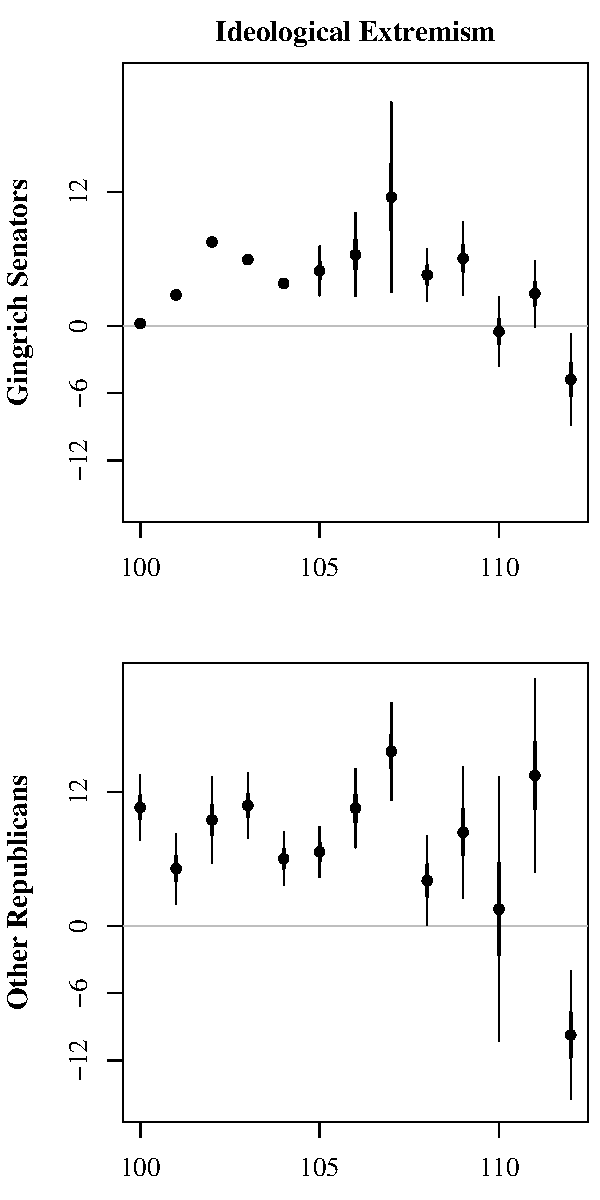
\includegraphics[width = 9cm]{C:/Users/Ethan/Documents/GitHub/partycalls/plots/senate-figure2-gingrich-other-reps.pdf}
\end{figure}

\begin{figure}[H]
	\centering
	\caption{Senate Ideological Extremism Coefficient Plot, Southern and Other Democrats}
	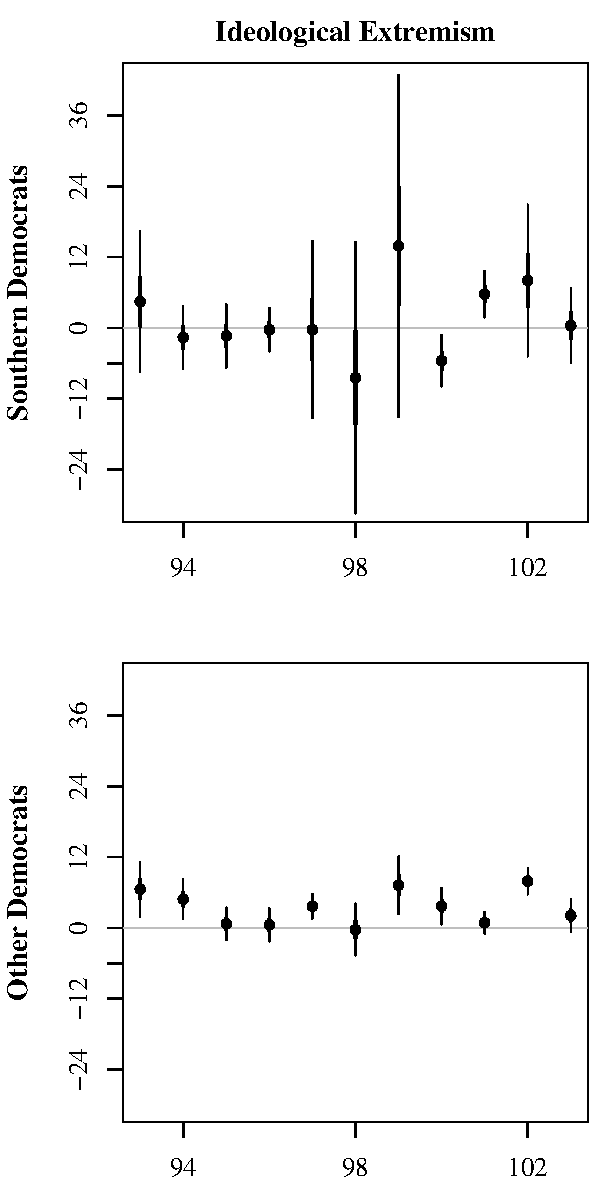
\includegraphics[width = 9cm]{C:/Users/Ethan/Documents/GitHub/partycalls/plots/senate-figure2-southern-other-dems.pdf}
\end{figure}

\subsection{DV/IV and IV/IV Plots by Reelection Status}

Since one of the main topics for the paper we are working on concerns reelection, in the following plots I show how both OLS and loess fit lines so we can better consider the nature of this particular relationship.

\begin{figure}[H]
	\centering
	\caption{Senate IV/IV Plot, Democrats, Re-election, Loess}
	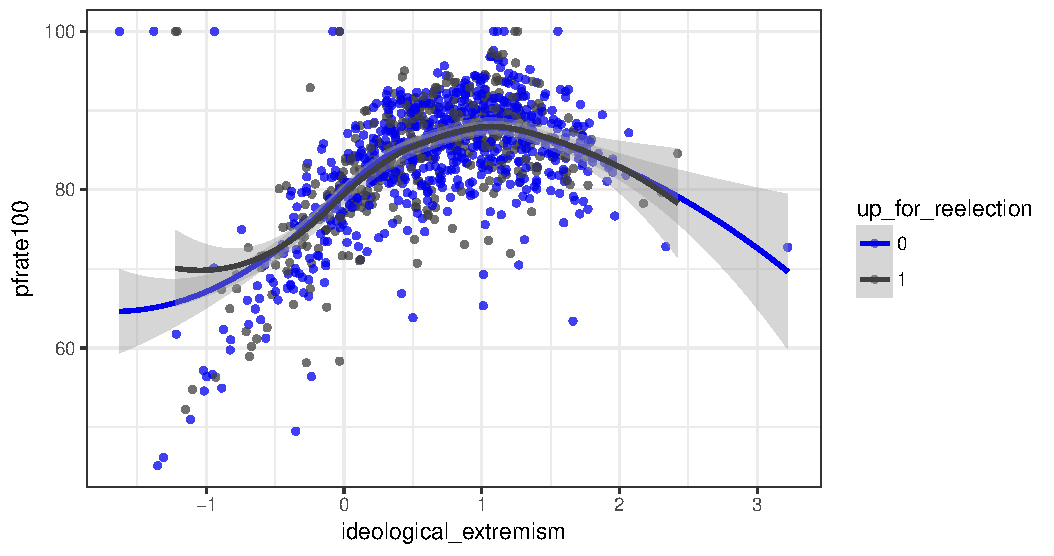
\includegraphics[width = \textwidth]{C:/Users/Ethan/Documents/GitHub/partycalls/plots/senate_dem_iv-iv_reelection_loess.pdf}
\end{figure}

\begin{figure}[H]
	\centering
	\caption{Senate IV/DV Plot, Democrats, Re-election, Loess}
	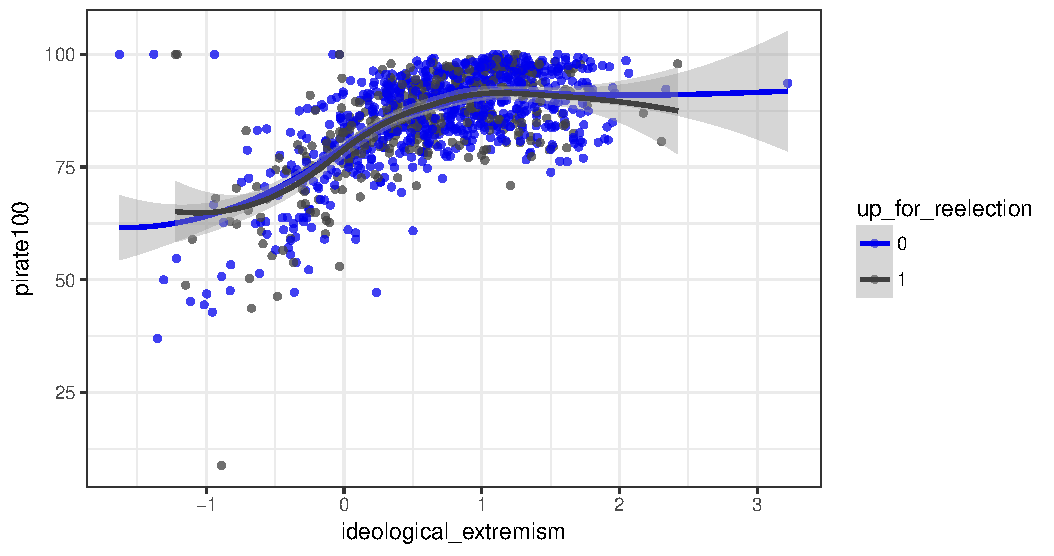
\includegraphics[width = \textwidth]{C:/Users/Ethan/Documents/GitHub/partycalls/plots/senate_dem_iv-dv_reelection_loess.pdf}
\end{figure}

\begin{figure}[H]
	\centering
	\caption{Senate IV/IV Plot, Democrats, Re-election, OLS}
	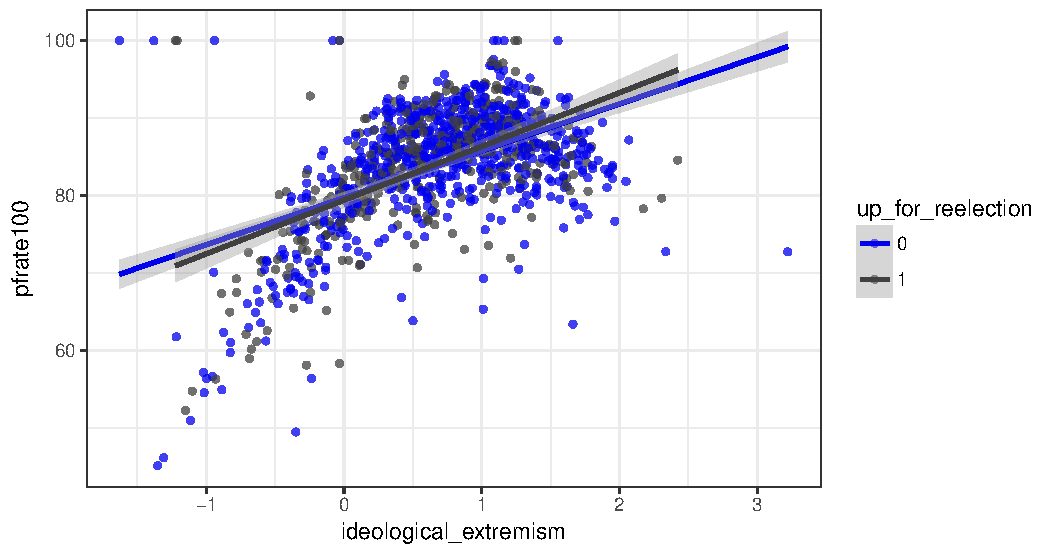
\includegraphics[width = \textwidth]{C:/Users/Ethan/Documents/GitHub/partycalls/plots/senate_dem_iv-iv_reelection_lm.pdf}
\end{figure}

\begin{figure}[H]
	\centering
	\caption{Senate IV/DV Plot, Democrats, Re-election, OLS}
	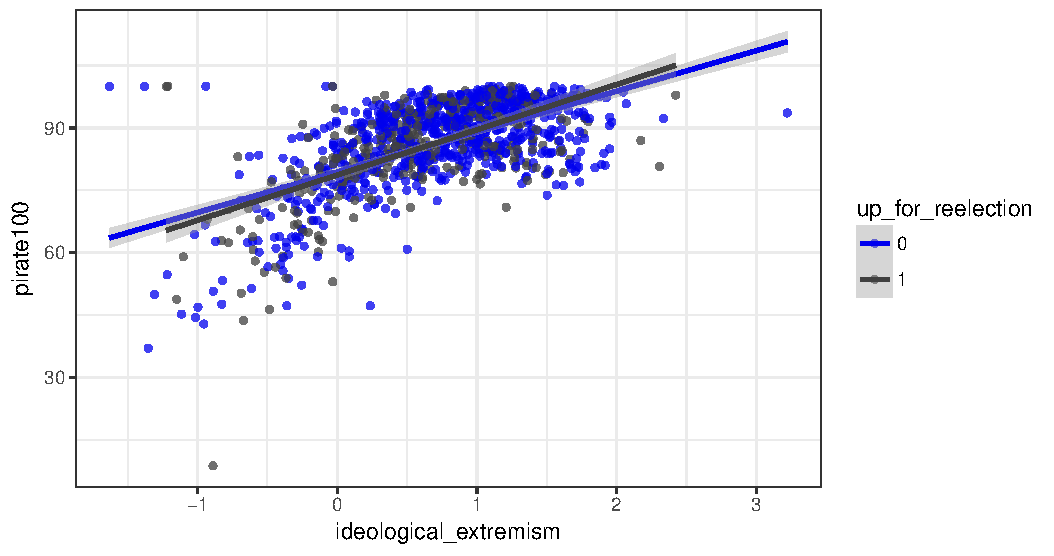
\includegraphics[width = \textwidth]{C:/Users/Ethan/Documents/GitHub/partycalls/plots/senate_dem_iv-dv_reelection_lm.pdf}
\end{figure}

\begin{figure}[H]
	\centering
	\caption{Senate IV/IV Plot, Republicans, Re-election, Loess}
	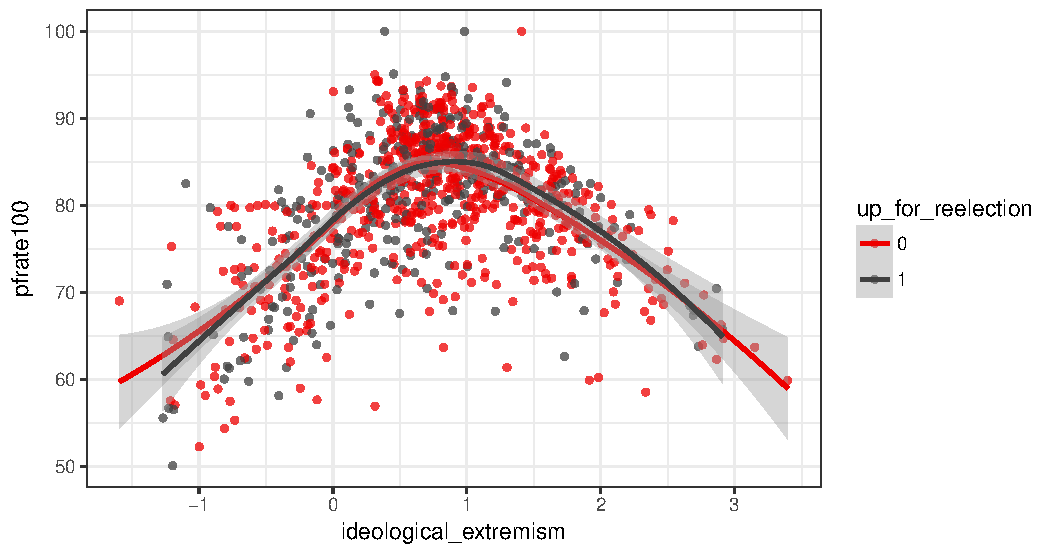
\includegraphics[width = \textwidth]{C:/Users/Ethan/Documents/GitHub/partycalls/plots/senate_rep_iv-iv_reelection_loess.pdf}
\end{figure}

\begin{figure}[H]
	\centering
	\caption{Senate IV/DV Plot, Republicans, Re-election, Loess}
	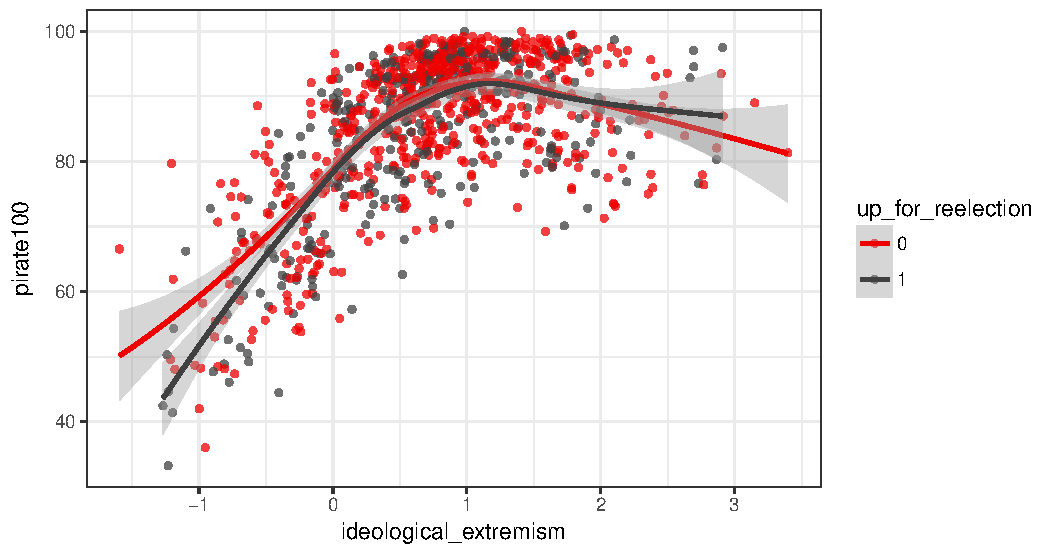
\includegraphics[width = \textwidth]{C:/Users/Ethan/Documents/GitHub/partycalls/plots/senate_rep_iv-dv_reelection_loess.pdf}
\end{figure}

\begin{figure}[H]
	\centering
	\caption{Senate IV/IV Plot, Republicans, Re-election, OLS}
	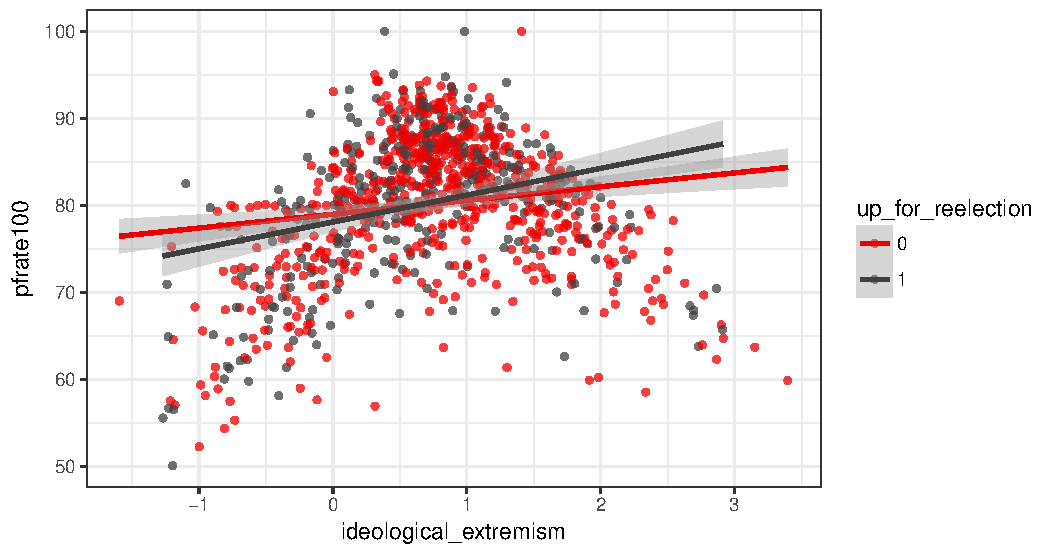
\includegraphics[width = \textwidth]{C:/Users/Ethan/Documents/GitHub/partycalls/plots/senate_rep_iv-iv_reelection_lm.pdf}
\end{figure}

\begin{figure}[H]
	\centering
	\caption{Senate IV/DV Plot, Republicans, Re-election, OLS}
	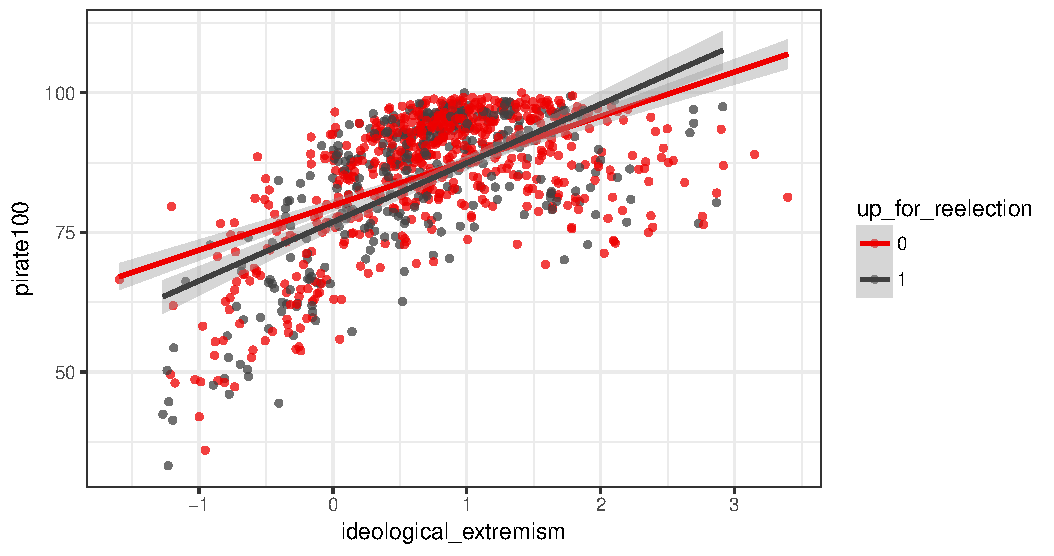
\includegraphics[width = \textwidth]{C:/Users/Ethan/Documents/GitHub/partycalls/plots/senate_rep_iv-dv_reelection_lm.pdf}
\end{figure}


\begin{figure}[H]
	\centering
	\caption{Senate IV/IV Plot, Majority Party, Re-election, Loess}
	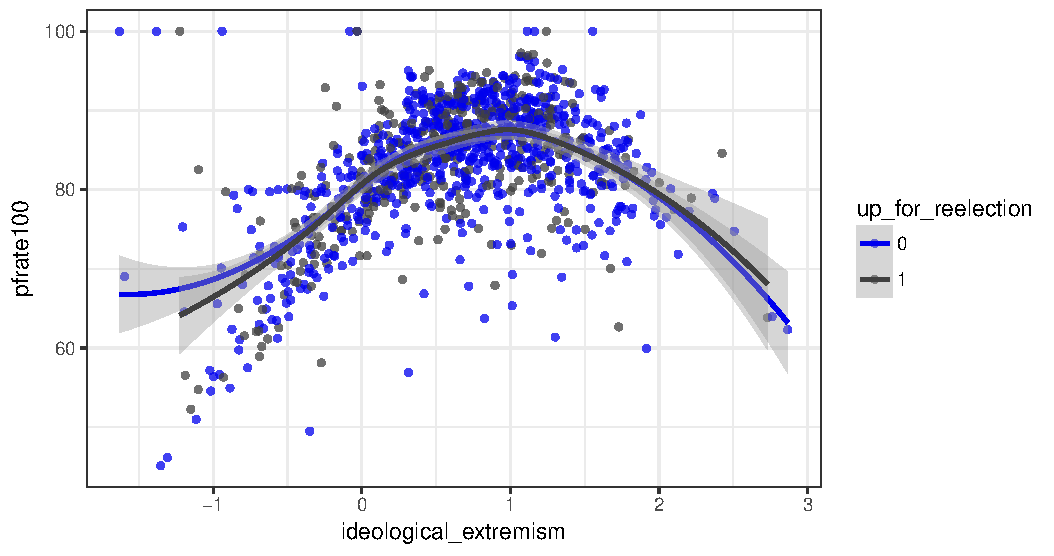
\includegraphics[width = \textwidth]{C:/Users/Ethan/Documents/GitHub/partycalls/plots/senate_maj_iv-iv_reelection_loess.pdf}
\end{figure}

\begin{figure}[H]
	\centering
	\caption{Senate IV/DV Plot, Majority Party, Re-election, Loess}
	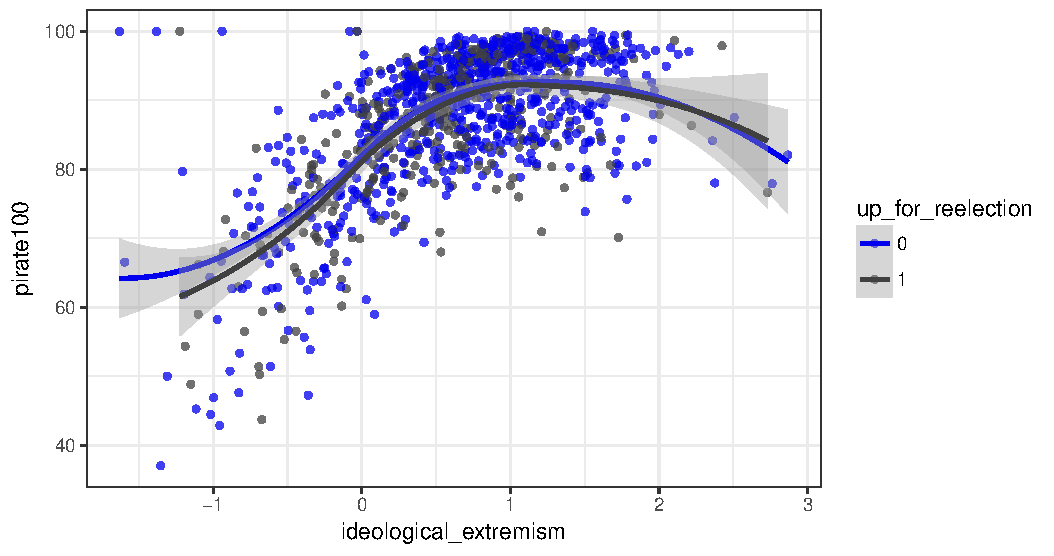
\includegraphics[width = \textwidth]{C:/Users/Ethan/Documents/GitHub/partycalls/plots/senate_maj_iv-dv_reelection_loess.pdf}
\end{figure}

\begin{figure}[H]
	\centering
	\caption{Senate IV/IV Plot, Majority Party, Re-election, OLS}
	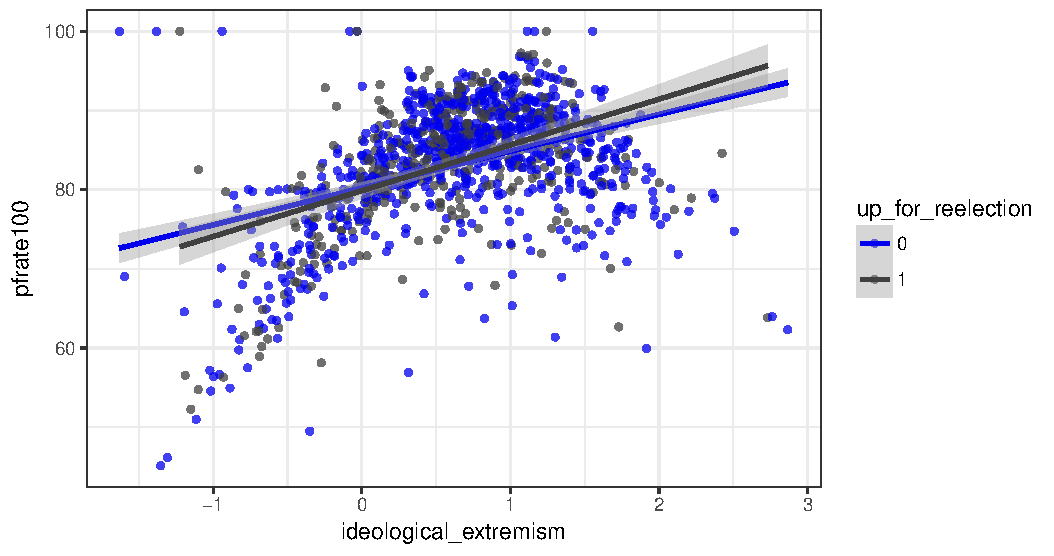
\includegraphics[width = \textwidth]{C:/Users/Ethan/Documents/GitHub/partycalls/plots/senate_maj_iv-iv_reelection_lm.pdf}
\end{figure}

\begin{figure}[H]
	\centering
	\caption{Senate IV/DV Plot, Majority Party, Re-election, OLS}
	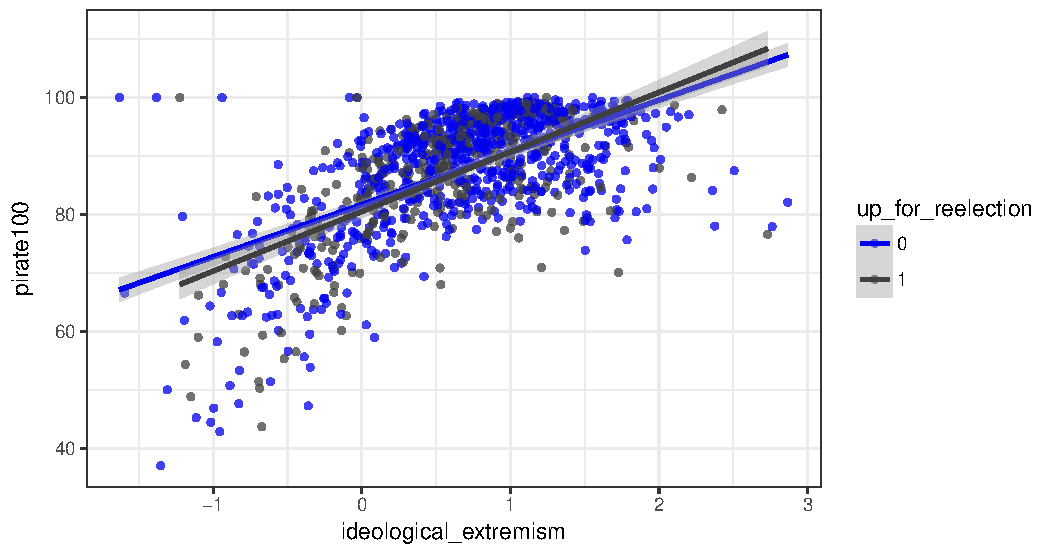
\includegraphics[width = \textwidth]{C:/Users/Ethan/Documents/GitHub/partycalls/plots/senate_maj_iv-dv_reelection_lm.pdf}
\end{figure}

\begin{figure}[H]
	\centering
	\caption{Senate IV/IV Plot, Minority Party, Re-election, Loess}
	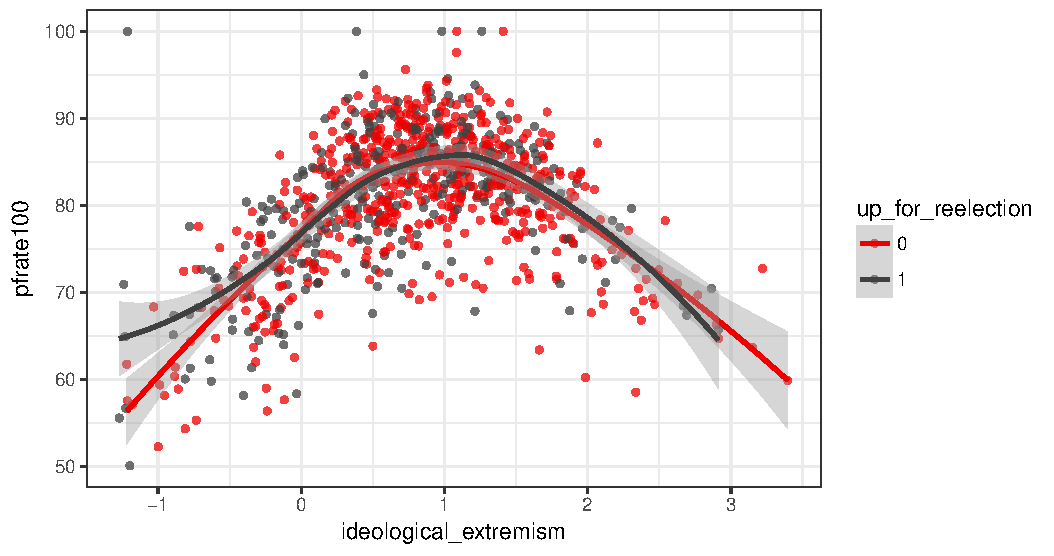
\includegraphics[width = \textwidth]{C:/Users/Ethan/Documents/GitHub/partycalls/plots/senate_min_iv-iv_reelection_loess.pdf}
\end{figure}

\begin{figure}[H]
	\centering
	\caption{Senate IV/DV Plot, Minority Party, Re-election, Loess}
	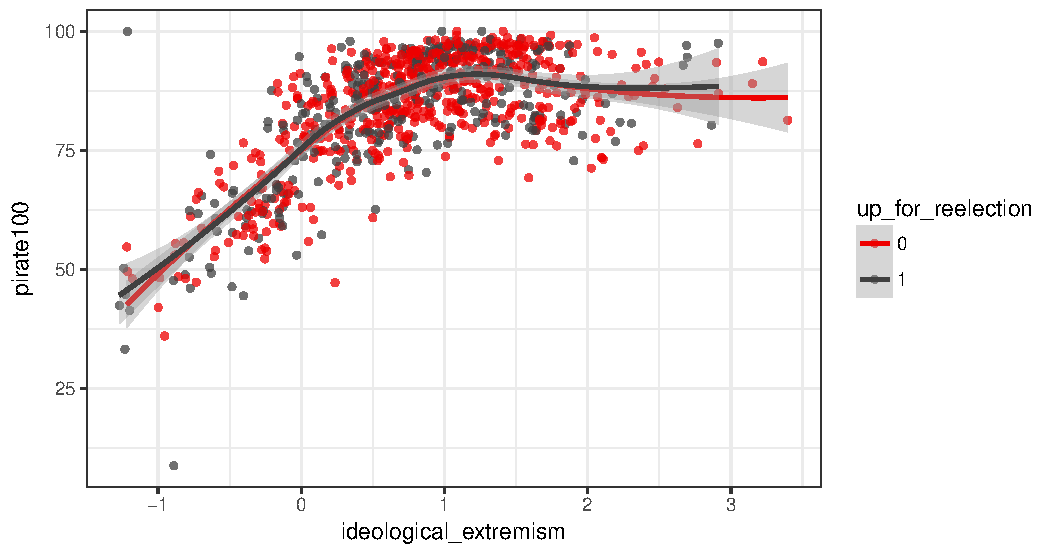
\includegraphics[width = \textwidth]{C:/Users/Ethan/Documents/GitHub/partycalls/plots/senate_min_iv-dv_reelection_loess.pdf}
\end{figure}

\begin{figure}[H]
	\centering
	\caption{Senate IV/IV Plot, Minority Party, Re-election, OLS}
	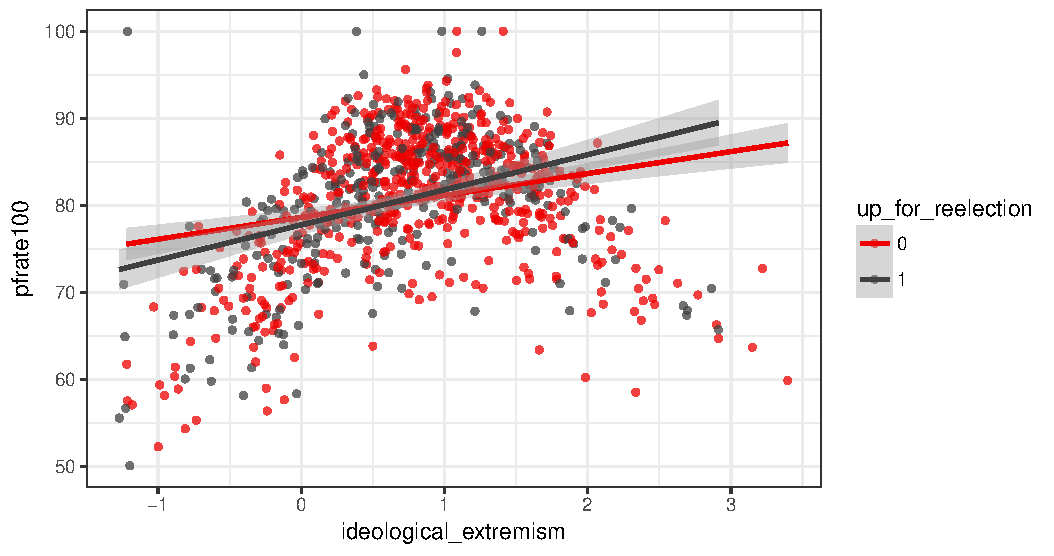
\includegraphics[width = \textwidth]{C:/Users/Ethan/Documents/GitHub/partycalls/plots/senate_min_iv-iv_reelection_lm.pdf}
\end{figure}

\begin{figure}[H]
	\centering
	\caption{Senate IV/DV Plot, Minority Party, Re-election, OLS}
	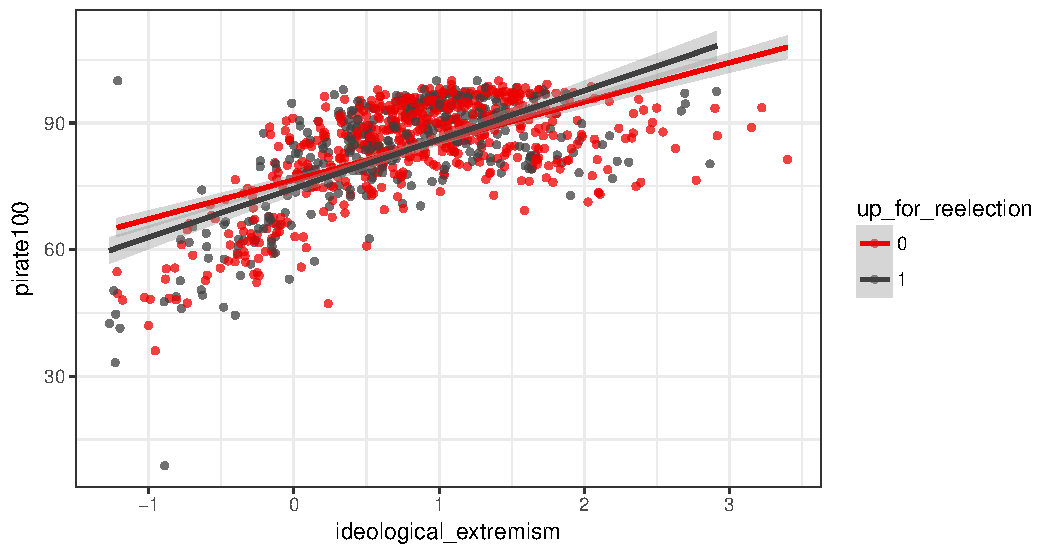
\includegraphics[width = \textwidth]{C:/Users/Ethan/Documents/GitHub/partycalls/plots/senate_min_iv-dv_reelection_lm.pdf}
\end{figure}

\begin{figure}[H]
	\centering
	\caption{Senate IV/IV Plot, Majority Democrats, Re-election, Loess}
	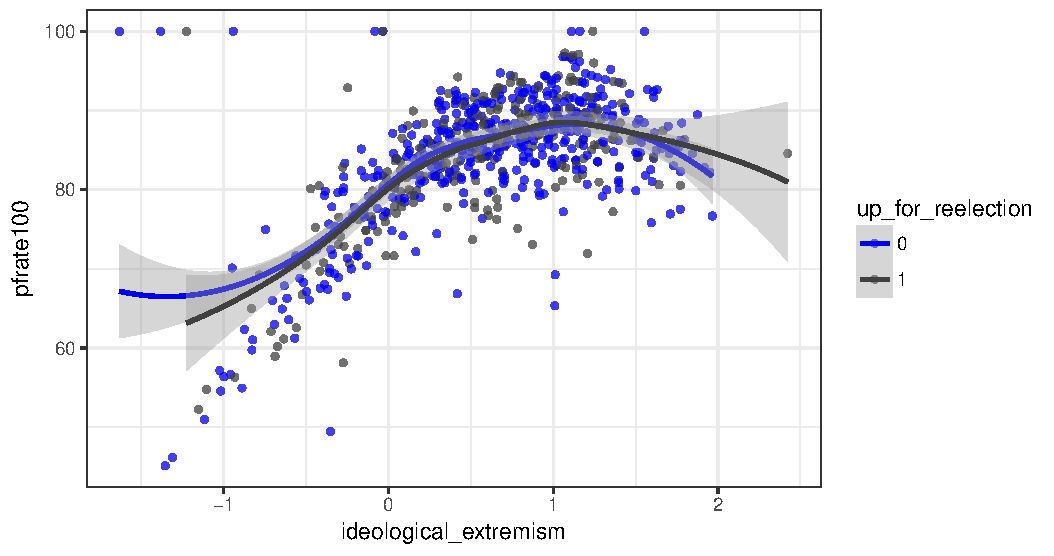
\includegraphics[width = \textwidth]{C:/Users/Ethan/Documents/GitHub/partycalls/plots/senate_maj_dem_iv-iv_reelection_loess.pdf}
\end{figure}

\begin{figure}[H]
	\centering
	\caption{Senate IV/DV Plot, Majority Democrats, Re-election, Loess}
	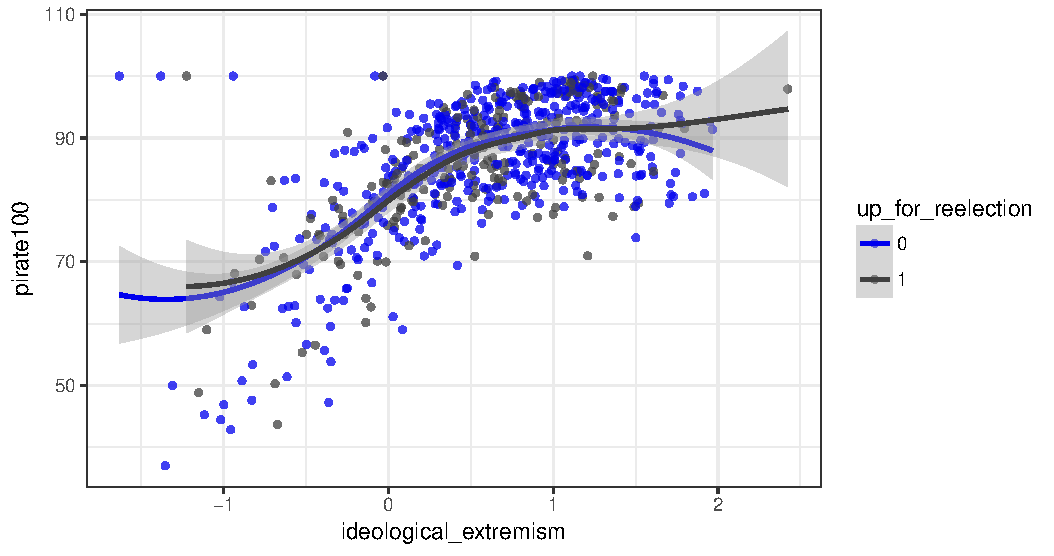
\includegraphics[width = \textwidth]{C:/Users/Ethan/Documents/GitHub/partycalls/plots/senate_maj_dem_iv-dv_reelection_loess.pdf}
\end{figure}

\begin{figure}[H]
	\centering
	\caption{Senate IV/IV Plot, Majority Democrats, Re-election, OLS}
	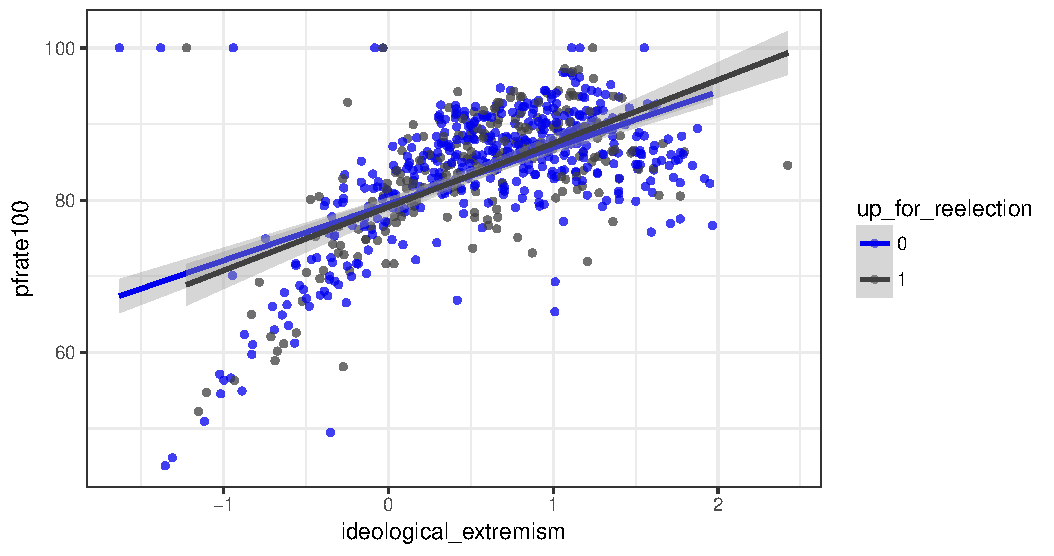
\includegraphics[width = \textwidth]{C:/Users/Ethan/Documents/GitHub/partycalls/plots/senate_maj_dem_iv-iv_reelection_lm.pdf}
\end{figure}

\begin{figure}[H]
	\centering
	\caption{Senate IV/DV Plot, Majority Democrats, Re-election, OLS}
	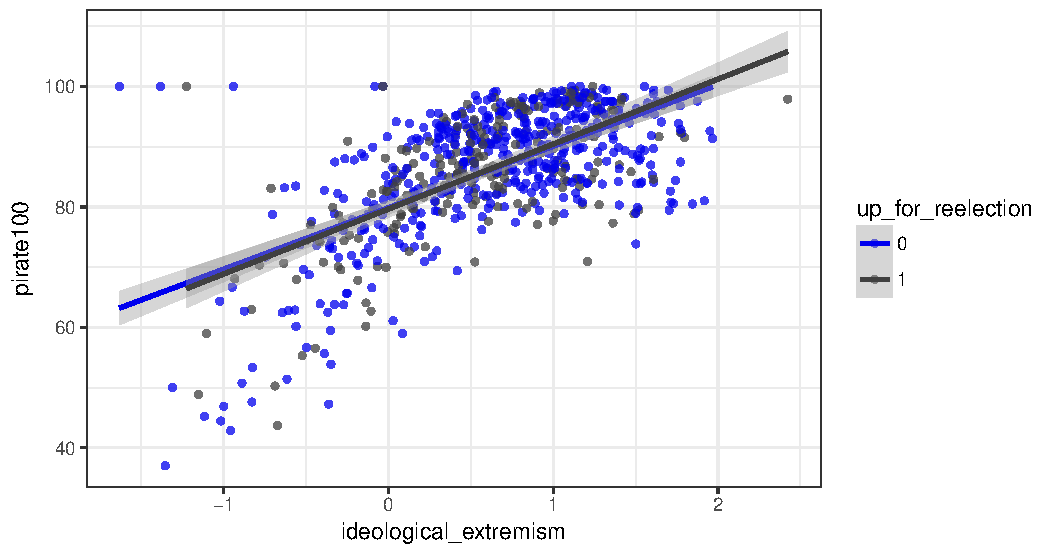
\includegraphics[width = \textwidth]{C:/Users/Ethan/Documents/GitHub/partycalls/plots/senate_maj_dem_iv-dv_reelection_lm.pdf}
\end{figure}

\begin{figure}[H]
	\centering
	\caption{Senate IV/IV Plot, Minority Democrats, Re-election, Loess}
	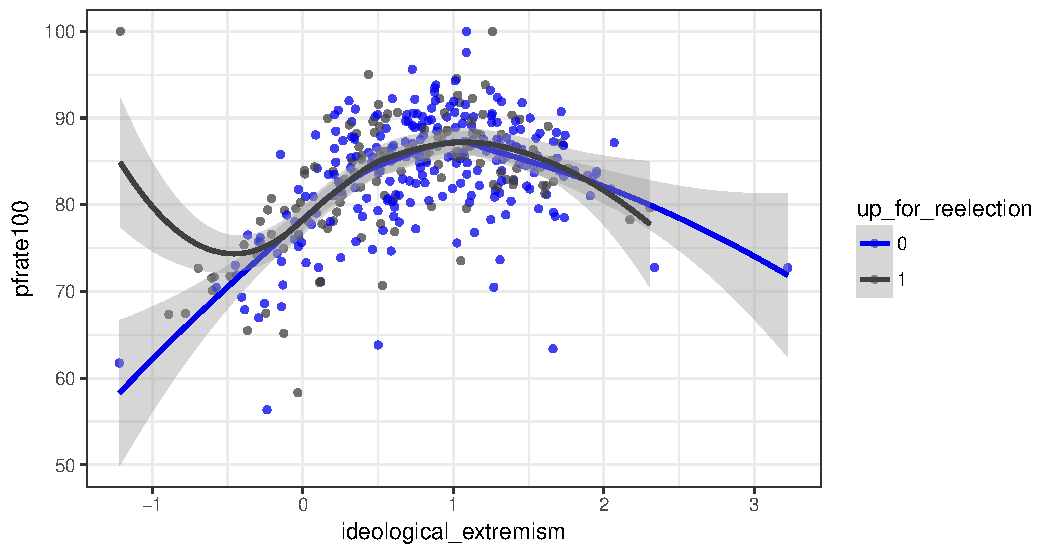
\includegraphics[width = \textwidth]{C:/Users/Ethan/Documents/GitHub/partycalls/plots/senate_min_dem_iv-iv_reelection_loess.pdf}
\end{figure}

\begin{figure}[H]
	\centering
	\caption{Senate IV/DV Plot, Minority Democrats, Re-election, Loess}
	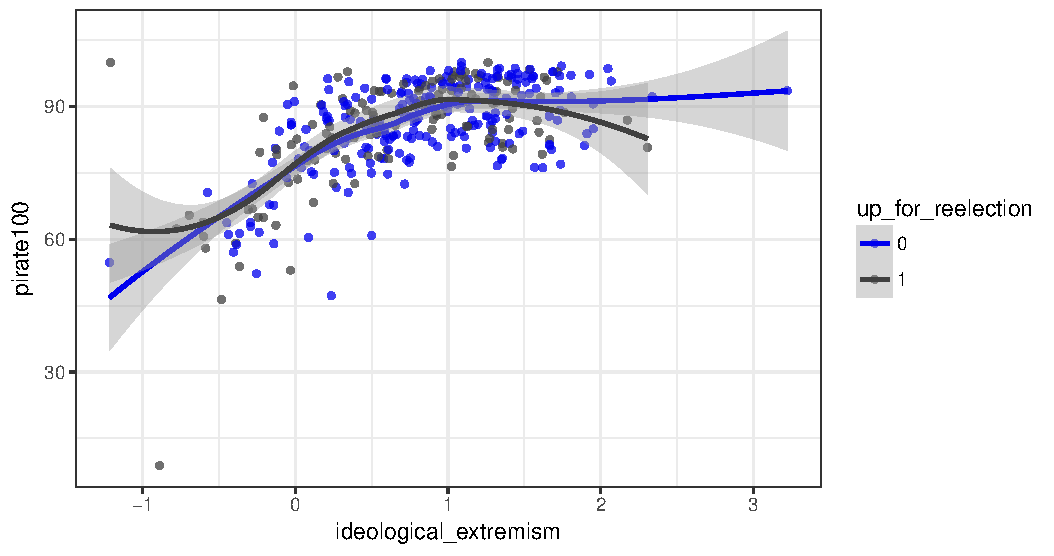
\includegraphics[width = \textwidth]{C:/Users/Ethan/Documents/GitHub/partycalls/plots/senate_min_dem_iv-dv_reelection_loess.pdf}
\end{figure}

\begin{figure}[H]
	\centering
	\caption{Senate IV/IV Plot, Minority Democrats, Re-election, OLS}
	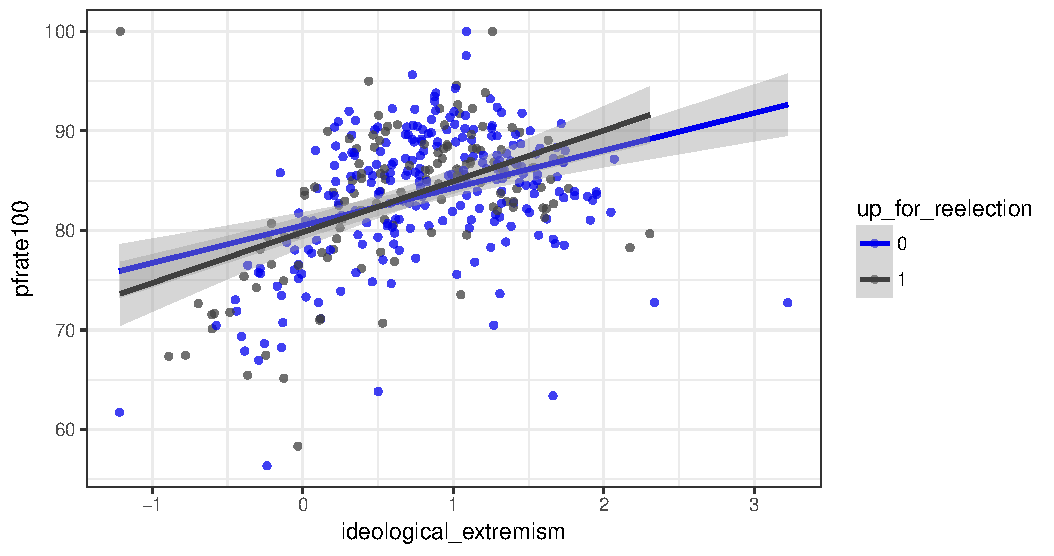
\includegraphics[width = \textwidth]{C:/Users/Ethan/Documents/GitHub/partycalls/plots/senate_min_dem_iv-iv_reelection_lm.pdf}
\end{figure}

\begin{figure}[H]
	\centering
	\caption{Senate IV/DV Plot, Minority Democrats, Re-election, OLS}
	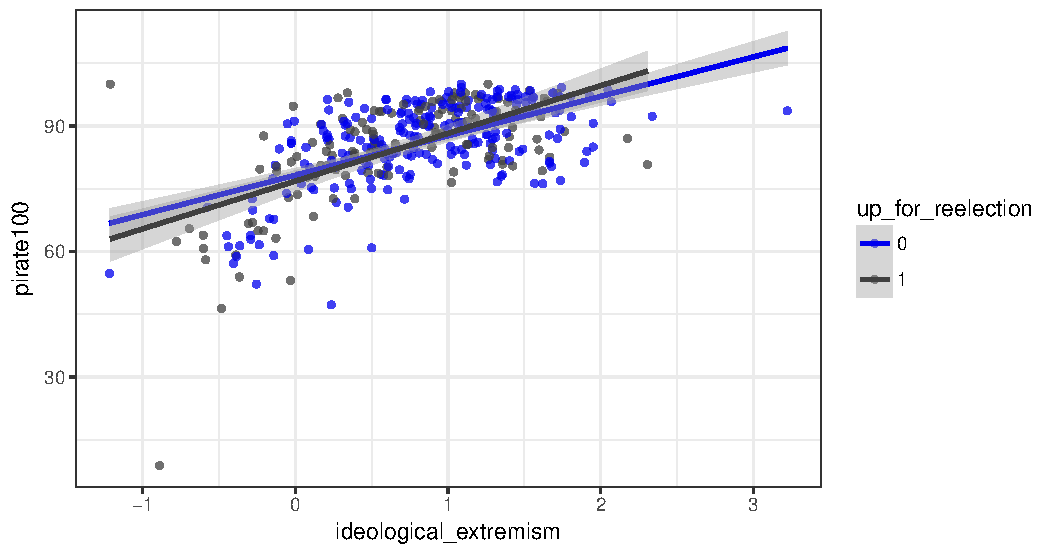
\includegraphics[width = \textwidth]{C:/Users/Ethan/Documents/GitHub/partycalls/plots/senate_min_dem_iv-dv_reelection_lm.pdf}
\end{figure}

\begin{figure}[H]
	\centering
	\caption{Senate IV/IV Plot, Majority Republicans, Re-election, Loess}
	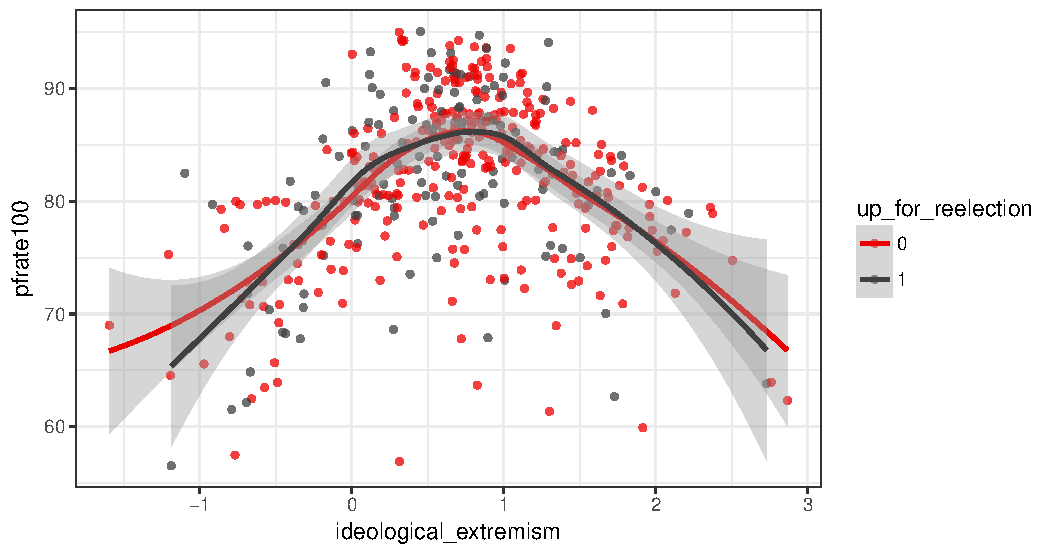
\includegraphics[width = \textwidth]{C:/Users/Ethan/Documents/GitHub/partycalls/plots/senate_maj_rep_iv-iv_reelection_loess.pdf}
\end{figure}

\begin{figure}[H]
	\centering
	\caption{Senate IV/DV Plot, Majority Republicans, Re-election, Loess}
	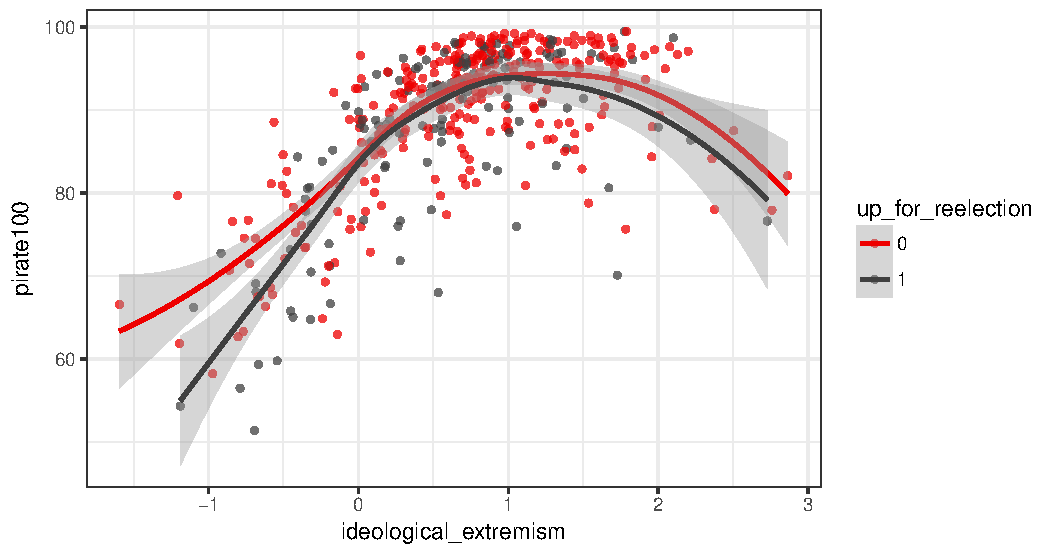
\includegraphics[width = \textwidth]{C:/Users/Ethan/Documents/GitHub/partycalls/plots/senate_maj_rep_iv-dv_reelection_loess.pdf}
\end{figure}

\begin{figure}[H]
	\centering
	\caption{Senate IV/IV Plot, Majority Republicans, Re-election, OLS}
	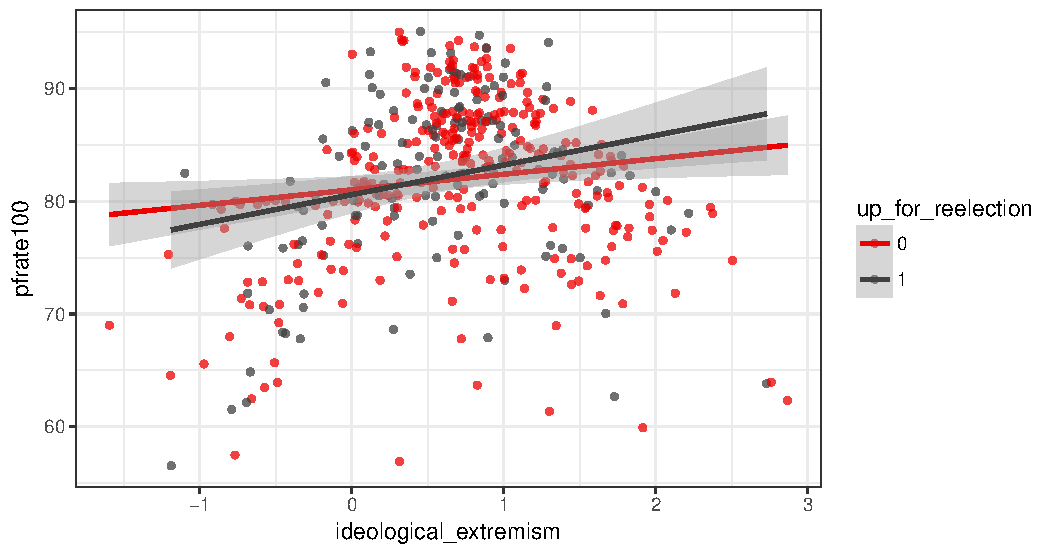
\includegraphics[width = \textwidth]{C:/Users/Ethan/Documents/GitHub/partycalls/plots/senate_maj_rep_iv-iv_reelection_lm.pdf}
\end{figure}

\begin{figure}[H]
	\centering
	\caption{Senate IV/DV Plot, Majority Republicans, Re-election, OLS}
	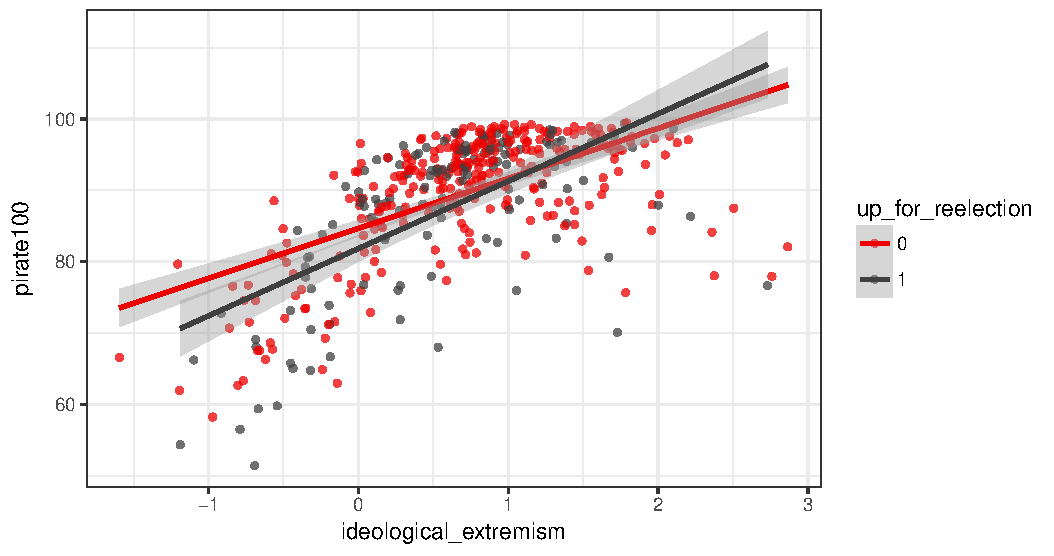
\includegraphics[width = \textwidth]{C:/Users/Ethan/Documents/GitHub/partycalls/plots/senate_maj_rep_iv-dv_reelection_lm.pdf}
\end{figure}

\begin{figure}[H]
	\centering
	\caption{Senate IV/IV Plot, Minority Republicans, Re-election, Loess}
	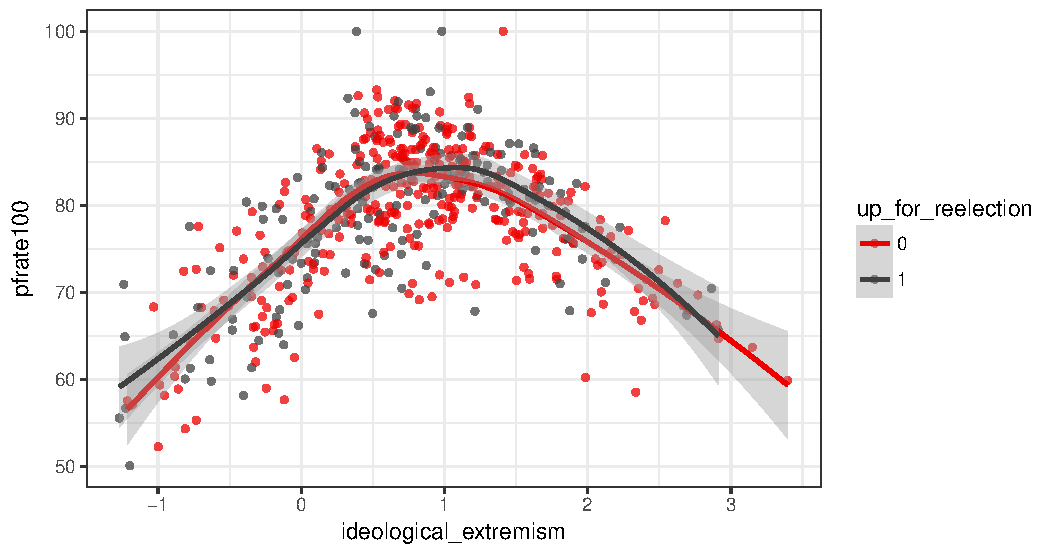
\includegraphics[width = \textwidth]{C:/Users/Ethan/Documents/GitHub/partycalls/plots/senate_min_rep_iv-iv_reelection_loess.pdf}
\end{figure}

\begin{figure}[H]
	\centering
	\caption{Senate IV/DV Plot, Minority Republicans, Re-election, Loess}
	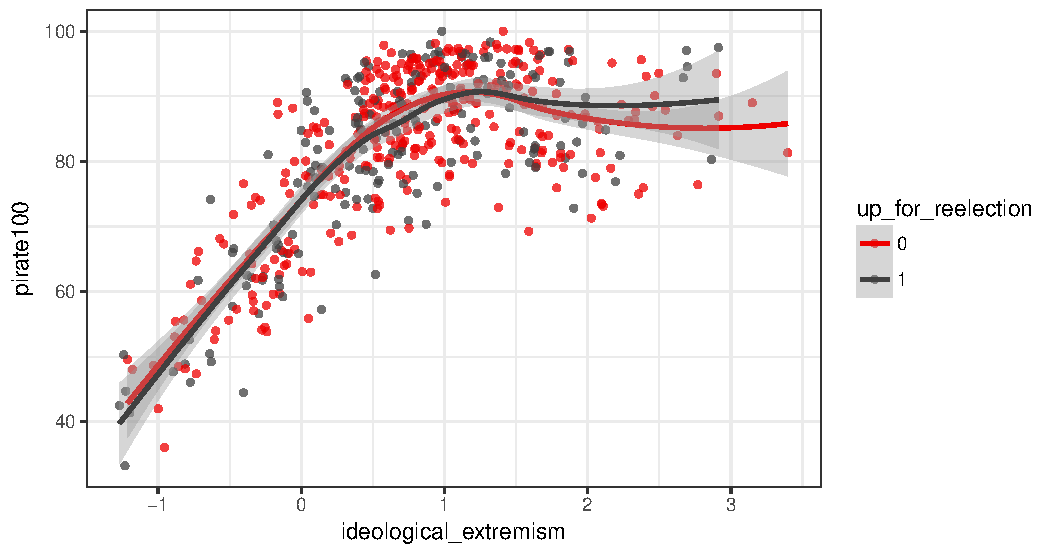
\includegraphics[width = \textwidth]{C:/Users/Ethan/Documents/GitHub/partycalls/plots/senate_min_rep_iv-dv_reelection_loess.pdf}
\end{figure}

\begin{figure}[H]
	\centering
	\caption{Senate IV/IV Plot, Minority Republicans, Re-election, OLS}
	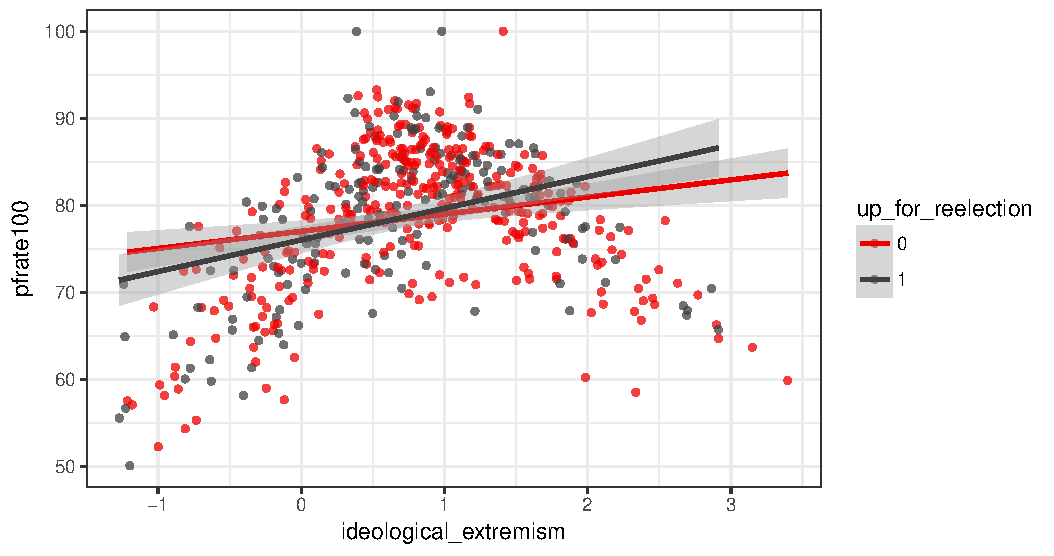
\includegraphics[width = \textwidth]{C:/Users/Ethan/Documents/GitHub/partycalls/plots/senate_min_rep_iv-iv_reelection_lm.pdf}
\end{figure}

\begin{figure}[H]
	\centering
	\caption{Senate IV/DV Plot, Minority Republicans, Re-election, OLS}
	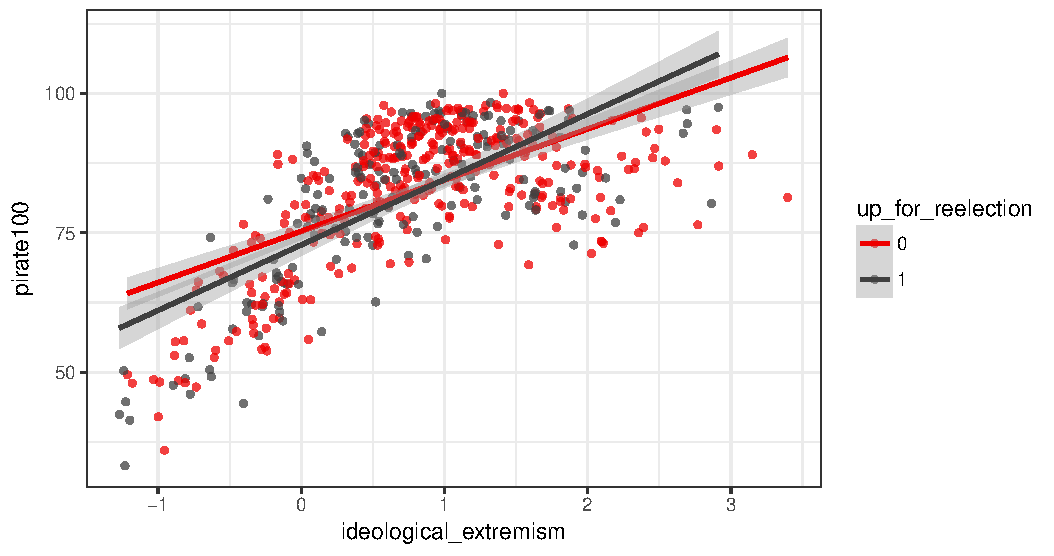
\includegraphics[width = \textwidth]{C:/Users/Ethan/Documents/GitHub/partycalls/plots/senate_min_rep_iv-dv_reelection_lm.pdf}
\end{figure}

































































\end{document}